% !TEX root = ../main_lecture_notes.tex
\chapter{Consensus protocol}\label{chap:consensus}
Transactions flow through the network of full nodes. After reviewing them, the full nodes must agree on the transaction that will be recorded in the next block. to do this, an algorithm must be designed so that consensus is reached.
A consensus protocol must be based on one of the scarce resources available to the network peers which include
\begin{itemize}
	\item bandwidth
	\item computational power
	\item storage 
\end{itemize}
The first solution that comes to mind for reaching consensus is a majority vote based on a message exchange system. This solution has been proposed by \citet{lamport1982the} within the famous "Byzantine general problem". A voting system inside a large network involves a colossal number of messages exchanged leading to the consumption of all the bandwidth, the failure of some nodes by denial of service and delays in the synchronization of the network. Practical solution like the celebrated Practical Byzantine Fault Tolerance (PBFT) presented in \citet{10.5555/296806.296824} have been implemented in some blockchain systems. Despite these advances, a change in methods was needed to accommodate a network that could grow indefinitely.\\

\noindent \citet{Na08} solved this scaling problem by proposing a system based on the election of a leader. The Proof-of-Work (\PoW) protocol appoints a leader based on its computing resources. Each node competes to solve a puzzle with a brute force search algorithm. The first node who is able to propose a solution append the next block. The search for a solution, referred to as mining, is associated with an operational cost borne by the nodes which is compensated by a reward expressed in the native blockchain cryptocurrency. The surge in cryptocurrency prices has led to a rush in block mining, leading to a major spike in the electricity consumption and electronic waste generation of blockchain networks. The blockchain network consumes as much electricity as countries the size of Thailand at the time of the writing. The need for a more environmentally friendly consensus protocol therefore becomes pivotal. Protocol such as \textit{Proof-of-Capacity} and \textit{Proof-of-Spacetime} use storage. Using storage is seen as a fairer and greener alternative by blockchain enthusiasts due to the general purpose nature of storage and the lower energy cost required by storage. The fact that most storage resources are owned by companies offering cloud storage solution poses a threat to the decentralized nature of the distributed ledger. The Proof-of-Interaction (\PoI) protocol, proposed by \citet{Abegg2021}, takes as leader the first node that is able to contact and obtain a response from a random sequence of nodes. This is a bandwidth-based alternative that is more scalable than majority voting. Along with bandwidth, computing power, and storage, a new resource has emerged with the advent of cryptocurrencies as a medium of exchange. The Proof-of-Stake protocol, described by \citet{Saleh2020}, selects a node with a probability proportional to the number of cryptocoins it holds. \\

\noindent The consensus protocol are applied so that a blocks are appended sequentially and not at the same time. Usually the consensus process is divided into time slots, also called rounds. The block generation time must be higher than the propagation delay in the network. If two blocks are created at the same time then a fork will occur. Two branches of the blockchain co-exists. A fork situation then resolves by applying the \textit{Longest Chain Rule} (LCR).
\begin{definition}
The \textit{Longest Chain Rule} states that if there exist several branches of the blockchain tehn the longest should be trusted.
\end{definition}  
\noindent This definition implies that a threshold must be chosen in order to decide when shorter branches of the blockchain should be discarded. For instance, a branch can be considered legitimate if it is $k\in\mathbb{N}$ blocks ahead of its pursuers.
For the consensus protocol to be viable, nodes must be incentivized to follow the LCR.\\

\noindent This chapter is organized as follows. \cref{sec:voting} gives a brief description of the voting based ways to get consensus by reviewing the "generals" problem. \cref{sec:leader} goes through the leader based consensus protocols, including \PoW in \cref{ssec:pow}, \PoSp in \cref{ssec:posp}, \PoI in \cref{ssec:poi}, and \PoS in \cref{ssec:pos}. For an exhaustive list of the existing protocols the reader is referred to \href{https://tokens-economy.gitbook.io/consensus/}{https://tokens-economy.gitbook.io/consensus/}.

\section{Voting system}\label{sec:voting} 
The problem of reaching consensus in a peer-to-peer network via a majority vote has been abstractedly compared to generals who must agree on a common battle plan. We start from the simple two general case before moving on the the situation of interest with several ones.
\subsection{Two generals problem}
Two generals wish to attack a city but they must agree on a timing to attack a city. They communicate via a messenger who must cross enemy territory at the risk of being intercepted. The first general $G_1$ sends a message to the second one $G_2$ saying 
$$
\texttt{"I will attack tomorrow at dawn"}
$$
For the attack to succeed, both generals must attack at the same time. Because their communication medium is unreliable, then $G_1$ must await confirmation from $G_2$ in order to attack. If $G_1$ does not receive confirmation then she will not attack. $G_2$ is aware of that and respond 
$$
\texttt{"I will follow your lead"}
$$
$G_2$ does not know whether the message went through and must wait for confirmation. This creates an infinite loop of messages and response, as on \cref{fig:message_loop}.
\begin{figure}[ht!]
 \begin{center}
\begin{tikzpicture}[->, >=stealth', auto, semithick, node distance=3cm]
\tikzstyle{every state}=[fill=white,draw=black,thick,text=black,scale=0.8]
\node[state]    (1)                     {$G_1$};
\node[state]    (2)[right of=1]   {$G_2$};
\path
(1) edge[bend left]     node{Attack}     (2)
(2) edge[bend left]     node{Confirmation}      (1);
\end{tikzpicture}
\end{center}
\caption{Message and confirmation loop}
\label{fig:message_loop}
\end{figure}
The two general problem is deemed unsolvable from a theoretical point of view and corresponds to a situation where two nodes communicate through an unreliable link. A practical solution for generals is to send many messengers hoping that at least one of them will succeed. This is only a thought experiment leading to the several general problem. 
\subsection{Byzantine General problem}
The blockchain network contains more than two nodes, these nodes must agree on the transactions to confirm. In a permissionless blockchain the nodes do not trust each other. The problem of the previous section generalizes to more than two generals, assuming that some generals are traitors which corresponds to faulty nodes in the network. This problem is referred to as The "Byzantine general problem" and was coined by \citet{lamport1982the}. Assume that $n>2$ generals must agree on a common battle plan for instance "Attack" (A) or "Retreat" (R) and that they can only communicate by two party messages. Denote by $m(i,j)$ the message sent by general $i$ to general $j$. Each general $j$ receives $n-1$ messages and applies a function $f$ to determine the course of action, for instance
$$
f(\{m(i,j);\text{ }i = 1,\ldots,n\}) = \begin{cases}
A,& \text{if }\sum_{i = 1}^n\mathbb{I}_{m(i,j) =A} >n/2,\\
R, &\text{else}.
\end{cases}
$$
If there are no traitors, each general is communicating the same value to all the peers and consensus is reached as in \cref{fig:no_traitor}. If one general is traitor, then he might not communicate the same value to all the generals and no consensus can be reached. It is the case for $G_4$ in \cref{fig:_one_traitor}.
\begin{figure}[!ht]
 \begin{center}
 \subfloat[No traitor]{
\begin{tikzpicture}[->, >=stealth', auto, semithick, node distance=2cm]
\tikzstyle{every state}=[fill=white,draw=black,thick,text=black,scale=0.8]
\node[state]    (1)                     {$G_1$};
\node[state]    (2)[below of=1]   {$G_2$};
\node[state]    (3)[below of=2]   {$G_3$};
\node[state]    (4)[below of=3]   {$G_4$};
\node[state]    (5)[below of=4]   {$G_5$};
\node[draw] (6) [right of=1]   {$f({A,R,R,A,A}) = A$};
\node[draw] (7) [right of=2]   {$f({A,R,R,A,A}) = A$};
\node[draw] (8) [right of=3]   {$f({A,R,R,A,A}) = A$};
\node[draw] (9) [right of=
4]   {$f({A,R,R,A,A}) = A$};
\node[draw] (10) [right of=5]   {$f({A,R,R,A,A}) = A$};
\path
(1) edge[bend left]     node{A}     (2)
(2) edge[bend left]     node{R}      (1)
(2) edge[bend left]     node{R}      (3)
(3) edge[bend left]     node{R}      (2)
(3) edge[bend left]     node{R}      (4)
(4) edge[bend left]     node{A}      (3)
(4) edge[bend left]     node{A}      (5)
(5) edge[bend left]     node{A}      (4)
;
\path
(1) edge     (6)
(2) edge     (7)
(3) edge     (8)
(4) edge     (9)
(5) edge     (10)
;
\end{tikzpicture}
\label{fig:no_traitor}}
\hskip2em
 \subfloat[One traitor]{
\begin{tikzpicture}[->, >=stealth', auto, semithick, node distance=2cm]
\tikzstyle{every state}=[fill=white,draw=black,thick,text=black,scale=0.8]
\node[state]    (1)                     {$G_1$};
\node[state]    (2)[below of=1]   {$G_2$};
\node[state]    (3)[below of=2]   {$G_3$};
\node[state]    (4)[below of=3]   {\color{red}$G_4$};
\node[state]    (5)[below of=4]   {$G_5$};
\node[draw] (6) [right of=1]   {$f({A,R,R,R,A}) = R$};
\node[draw] (7) [right of=2]   {$f({A,R,R,R,A}) = R$};
\node[draw] (8) [right of=3]   {$f({A,R,R,R,A}) = R$};
\node[draw] (9) [right of=
4]   {$f({A,R,R,?,A}) = ?$};
\node[draw] (10) [right of=5]   {$f({A,R,R,A,A}) = A$};
\path
(1) edge[bend left]     node{A}     (2)
(2) edge[bend left]     node{R}      (1)
(2) edge[bend left]     node{R}      (3)
(3) edge[bend left]     node{R}      (2)
(3) edge[bend left]     node{R}      (4)
(4) edge[bend left]     node{\color{red}R}      (3)
(4) edge[bend left]     node{\color{red}A}      (5)
(5) edge[bend left]     node{A}      (4)
;
\path
(1) edge     (6)
(2) edge     (7)
(3) edge     (8)
(4) edge     (9)
(5) edge     (10)
;
\end{tikzpicture}
\label{fig:_one_traitor}}
\end{center}
\caption{Majority vote with or without a traitor}
\label{fig:majority_vote}
\end{figure}
To handle such a situation, roles are given to the general. One of them become the leader and the other are the lieutenants. We aim at finding an algorithm such that
\begin{itemize}
	\item[C1] All the loyal lieutenants obey the same order
	\item[C2] If the commanding general is loyal, then  every loyal lieutenants obey the order he sends
\end{itemize}

A first result from \citet{lamport1982the} is the following
\begin{theo}
There are no solution to the Byzantine General problem for $n<3m+1$ generals where $m$ is the number of traitors.
\end{theo}
\begin{proof}
Consider the situation where $n = 3$ and $m = 1$. The traitor is either the commander or one of the lieutenants as shown in 
\begin{figure}[!ht]
 \begin{center}
 \subfloat[Commander is loyal]{
\begin{tikzpicture}[->, >=stealth', auto, semithick, node distance=4cm]
\tikzstyle{every state}=[fill=white,draw=black,thick,text=black,scale=0.8]
\node[state]    (1)               {C};
\node[state]    (2)[below left of=1]   {L1};
\node[state]    (3)[below right of=1]   {\begin{color}{red}L2 \end{color}};
\path
(1) edge[bend left]     node{A}     (3)
(1) edge[bend right]     node{A}      (2)
(2) edge[bend left]     node{A}      (3)
(3) edge[bend left]     node{R}      (2)
% (3) edge[bend left]     node{R}      (4)
% (4) edge[bend left]     node{A}      (3)
% (4) edge[bend left]     node{A}      (5)
% (5) edge[bend left]     node{A}      (4)
;
\end{tikzpicture}
\label{fig:commander_loyal}}
\hskip2em
\subfloat[Commander is a traitor]{
\begin{tikzpicture}[->, >=stealth', auto, semithick, node distance=4cm]
\tikzstyle{every state}=[fill=white,draw=black,thick,text=black,scale=0.8]
\node[state]    (1)               {\begin{color}{red}C \end{color}};
\node[state]    (2)[below left of=1]   {L1};
\node[state]    (3)[below right of=1]   {L2};
\path
(1) edge[bend left]     node{A}     (3)
(1) edge[bend right]     node{R}      (2)
(2) edge[bend left]     node{R}      (3)
(3) edge[bend left]     node{A}      (2)
% (3) edge[bend left]     node{R}      (4)
% (4) edge[bend left]     node{A}      (3)
% (4) edge[bend left]     node{A}      (5)
% (5) edge[bend left]     node{A}      (4)
;
\end{tikzpicture}
\label{fig:commander_traitor}}
\end{center}
\caption{Majority vote with or without a traitor}
\label{fig:majority_vote}
\end{figure}
Unfortunately for Lieutenant 2, there is no way for her to tell apart the situation pictured in \cref{fig:commander_loyal} and \cref{fig:commander_traitor} and therefore no way to ensure both C1 and C2. We prove the result for $n>3$ by contradiction. Assume that there is a way to verify both C1 and C2 with $3<n<3m+1$. We then construct a solution with generals by having one general simulate the commander plus at most $m-1$ generals, and the other two simulating at most $m$ generals. One of the generals gather all the traitors and is therefore a traitor. The other two are loyal generals as they only simulate loyals general. We have built a solution with three generals that we know is impossible. 
\end{proof}
Now we need an algorithm that allows $n>3m+1$ generals to deal with $m$ traitors. The 'Oral Message' algorithm denoted by $\text{OM}(m)$ and summarized in \cref{alg:om} can handle $m$ traitors if the number of generals verifies $n>3m+1$.
\begin{algorithm}[!ht]
\caption{The Oral message algorithm $\text{OM}(m)$}\label{alg:om}
\begin{algorithmic}[1]
\If{$m=0$};
\For{$i =1 \to n-1$} 
\State Commander sends $v_i = v$ to lieutenant $i$ 
\State Lieutenant $i$ set their value to $v$
\EndFor
\EndIf
\If{$m>0$};
\For{$i =1 \to n-1$} 
\State Commander sends $v_i$ to lieutenant $i$ 
\State Lieutenant $i$ uses OM(m-1) to communicate $v_i$ to the $n-2$ lieutenants
\EndFor
\For{$i =1 \to n-1$} 
\State Lieutenant $i$ set their value to $f(v_1, \ldots, v_{n-1})$
\EndFor
\EndIf
\end{algorithmic}
\end{algorithm}
Before looking into the theoretical justification of $\text{OM}(m)$, let us illustrate the algorithm with an example.
\begin{ex}
Consider the situation where $n = 4$ and $m = 1$ shown in \cref{fig:OM_algorithm_illustration}. 
\begin{figure}[!ht]
 \begin{center}
 \subfloat[Commander is loyal]{
\begin{tikzpicture}[->, >=stealth', auto, semithick, node distance=4cm]
\tikzstyle{every state}=[fill=white,draw=black,thick,text=black,scale=0.8]
\node[state]    (1)               {C};
\node[state]    (2)[below left of=1]   {L1};
\node[state]    (3)[below of=1]   {L2};
\node[state]    (4)[below right of=1]   {\begin{color}{red}L3 \end{color}};
\path
(1) edge[bend right]     node{A}     (2)
(1) edge[bend left]     node{A}      (4)
(1) edge     node{A}      (3)
(2) edge[bend right, below]     node{A}      (3)
(3) edge[bend right, above]     node{A}      (2)
(4) edge[bend right, above]     node{R}      (3)
(3) edge[bend right, below]     node{A}      (4)
;
\end{tikzpicture}
\label{fig:commander_loyal_om}}
\hskip2em
\subfloat[Commander is a traitor]{
\begin{tikzpicture}[->, >=stealth', auto, semithick, node distance=4cm]
\tikzstyle{every state}=[fill=white,draw=black,thick,text=black,scale=0.8]
\node[state]    (1)               {\begin{color}{red}C \end{color}};
\node[state]    (2)[below left of=1]   {L1};
\node[state]    (3)[below of=1]   {L2};
\node[state]    (4)[below right of=1]   {L3};
\path
(1) edge[bend right]     node{A}     (2)
(1) edge[bend left]     node{R}      (4)
(1) edge     node{R}      (3)
(2) edge[bend right, below]     node{A}      (3)
(3) edge[bend right, above]     node{R}      (2)
(4) edge[bend right, above]     node{R}      (3)
(3) edge[bend right, below]     node{R}      (4)
;
\end{tikzpicture}
\label{fig:commander_traitor_om}}
\end{center}
\caption{Illustration of the \text{OM}(m) algorithm in the case where $n = 4$ and $m=1$.}
\label{fig:OM_algorithm_illustration}
\end{figure}
If the commander is loyal then one of the lieutenant is a traitor, see \cref{fig:commander_loyal_om}. The commander gives the order to attack to all the lieutenant $3$ tells the other that she heard retreat from the commander. The loyal lieutenants then apply the map $f$ to agree on their value 
$$
f(A,A,R) = A,
$$
which coresponds to the order the commander sent, hence IC1 and IC2 are satisfied. If the commander is a traitor as in \cref{fig:commander_traitor_om}, then he sends conflicting order to the lieutenant but after communicating the value they received to each other finally agree on the following value
$$
f(A,R,R) = R,
$$
hence IC1 is satisfied and IC2 can be ignored since the commander is a traitor.
\end{ex}
\begin{theo}
Algorithm $\text{OM}(m)$ satisfies conditions IC1 and IC2 if $n>3m+1$.
\end{theo}
\begin{proof}
The proof follows from simple induction.\\

\noindent First assume that the commander is loyal. For $m = 0$, the commanders simply sends the value $v$ to all the lieutenants and IC2 holds. Assume that $\text{OM}(m-1)$ works when the commader is loyal. The commander sends $v$ to all the lieutenants. The lieutenants then applies $OM(m-1)$. Because $n-1>2k + m-1$, then it follows from the induction hypothesis that each loyal lieutenants get the value $v$ for each of the loyal lieutenants $j$. The loyal lieutenants $n-1-m > 2k-1>m $ outnumber the traitorous lieutenants and therefore set their value to 
$$
f(v_1,\ldots, v_{n-1}) = v,
$$  
and both IC1 and IC follow.\\

\noindent Let us assume that the commander is a traitor, we only have to worry about IC1 in that case. There are at most $m$ traitors and the commander is one of them. We therefore have $m-1$ traitors among the lieutenants. Since the total number of lieutenants exceeds three times the number of traitors $n-1>3m>3(m-1)$ then by applying $\text{OM}(m-1)$ all the loyal lieutenants receive the same vector of values $v_1,\ldots, v_{n-1}$, agree on the same value 
$$
f(v_1,\ldots,v_{n-1}) =v,
$$
which leads to the verification of IC1.
\end{proof}
The main problem associated to this Oral message algorithm is the number of messages is $n^{m+1}$ which is prohibitive for large values of $n$ and $m$. A celebrated algorithm, called Practical Byzantine Fault Tolerance (PBFT) has been developped later on by \citet{10.5555/296806.296824} but still not fast enough to enable the infinite growth of the network associated to public and permissionless blockchains.
\section{Leader system}\label{sec:leader}
The scalability issue can be solved by opting for a leader based mechanism instead of a majority vote mechanism. The protocols presented in this section use computational power, storage and bandwidth to elect a leader each time a new block must be appended to the blockchain.   
\subsection{Proof-of-Work}\label{ssec:pow}
The bitcoin blockchain relies on a consensus protocol based on computational power called Proof-of-Work (\PoW), presented in \citet{Na08}. A block consists of 
\begin{itemize}
\item a header 
\item a list of "transactions" that represents the information recorded through the blockchain. 
\end{itemize}
The header usually includes 
\begin{itemize}
\item the date and time of creation of the block, 
\item the block height which is the index inside the blockchain, 
\item the hash of the block 
\item the hash of the previous block. 
\end{itemize}
The hash of a block is obtained by concatenating the header and the transactions in a large character string thus forming a "message" denoted by $m$, to which a hash function $h$ is applied. 
\begin{definition}
A hash function is a function that can map data of arbitrary size to fixed-sized values, 
$$
h:\{0,1\}^\ast\mapsto \{0,1\}^d
$$ 
\end{definition}
The hash functions used in blockchain applications must be cryptographic, i.e.\ 
\begin{itemize}
\item quick to compute 
\item one way 
\item deterministic 
\end{itemize}
\begin{remark}
It must be nearly infeasible to generate a message with a given hash value or to find two messages with the same hash value. A small change in the message should change dramatically the hash value so that the new hash value appears to be uncorrelated to the previous hash, 
$$
\text{if }m_1\approx m_2\text{ then }h(m_1)\neq h(m_2).
$$ 
We will not expand on how to build such a cryptographic hash function, we refer the interested reader to the work of \citet{cryptoeprint:2011:565}. 
\end{remark}
In the bitcoin blockchain as well as in many other applications, the standard is the SHA-256 function which converts any message into a hash value of $256$ bits. The latter is usually translated into a hexadecimal digest, for instance the hash value of the title of the present manuscript reads as 
$$
\texttt{98b1146926548f6b57c4347457713ff2f035beda9c93f12fbc9b202e9c512e80}.
$$
Mining a block means finding a block hash value lower than some target which can only be achieved by brute force search thanks to the properties of cryptographic hash functions. In practice, the search for an appropriate hash value, referred to as a solution, is done by appending a nonce to the block message before applying the hash function. A nonce is a $32$ bits number, drawn at random by miners until a nonce resulting in a proper block hash value is found. For illustration, consider the block in Figure \ref{fig:block_not_mined}.

\begin{figure}[!ht]
		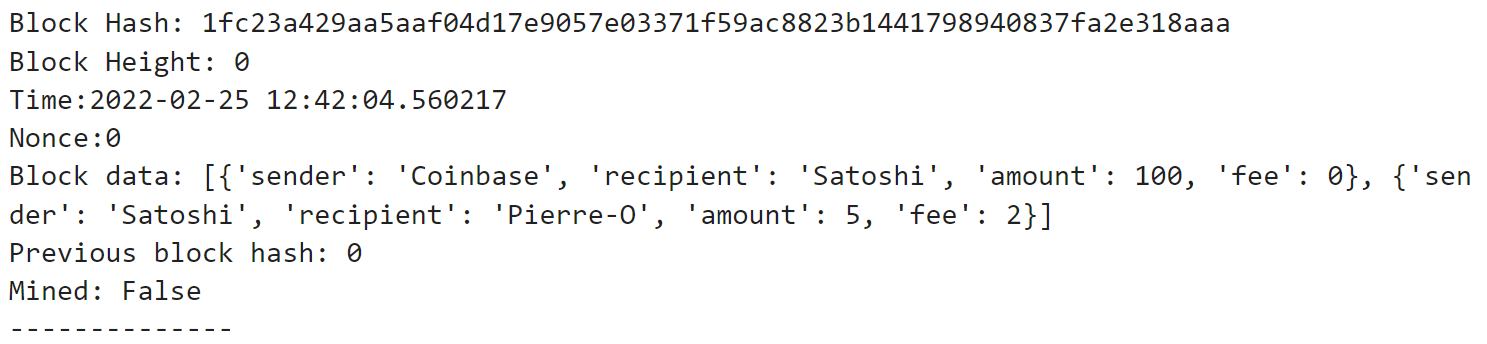
\includegraphics[width = \textwidth]{../Figures/block_not_mined.png}
		\captionsetup{width=0.8\textwidth}
		\centering
		\caption{A block that has not been mined yet.}
		\label{fig:block_not_mined}
\end{figure}
The hash value in decimal notation is $1.43e^{76}$ while the maximum value for a $256$ bits number is $2^{256}-1 \approx 1.16e^{77}$. We refer to the latter as the maximal target and denote it by $T_{\max}$. The Proof-of-Work protocol sets a target $T < T_{\max}$ and ask miners to find a nonce such that the hash value of the block is smaller than $T$. Practitioners would rather talk about the \textit{difficulty} which is defined as $D = T_{\max} / T$. If the difficulty is one, any hash value is acceptable. Increasing the difficulty reduces the set of allowable hash values, making the problem harder to solve. A hash value is then called \textit{acceptable} if its hexadecimal digest starts with a given number of zeros. If we set the difficulty to $2^4$, then the hexadecimal digest of the hash of the block must start with at least $1$ leading zero, making the hash value of the block in Figure \ref{fig:block_not_mined} not acceptable. After completing the nonce search we get the block in Figure \ref{fig:block_mined}.
\begin{figure}[!ht]
		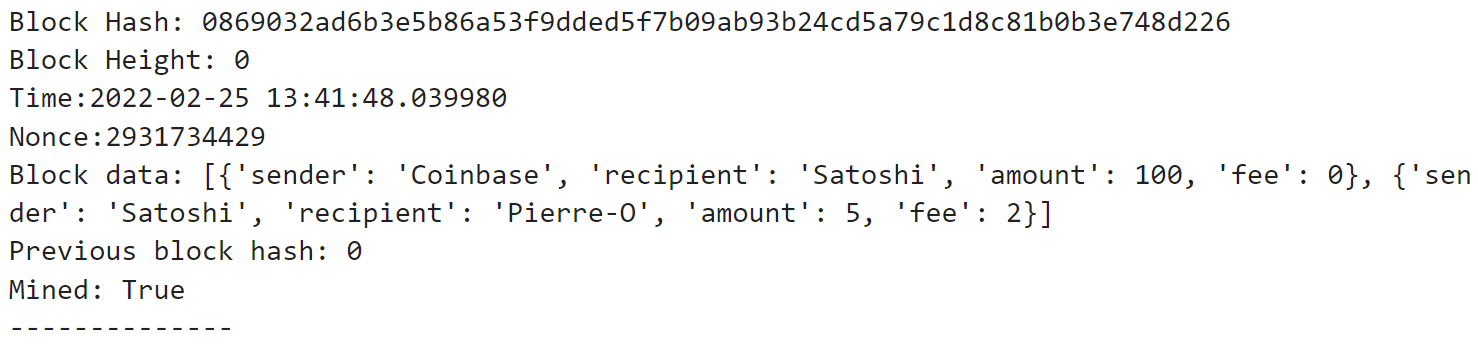
\includegraphics[width = \textwidth]{../Figures/block_mined.png}
		\captionsetup{width=0.8\textwidth}
		\centering
		\caption{A mined block with a hash value having on leading zero.}
		\label{fig:block_mined}
\end{figure}
Note that it took $5$ attempts to find this nonce. The number of needed trials is geometrically distributed with parameter $1 / D$, which means that with a difficulty of $D = 2^4$ it takes on average $16$ trials. The protocol adjusts the difficulty automatically every $2,016$ block discoveries so as to (globally) maintain one block discovery every $10$ minutes on average. The time between two block discoveries depends on the number of hash values computed by the network at a given instant. At the time of writing, the network computes $182.58$ Exahashes per second and the difficulty is $27,967,152,532,434$.\footnote{Source: \href{https://www.bitcoinblockhalf.com/}{bitcoinblockhalf.com}} For an exhaustive overview of the mining process in the bitcoin blockchain, we refer the reader to the book of \citet[Chapter 10]{Antonopoulos2017}. As each trial (of the system) for mining a block is
independent of the others and leads to a success with very small probability, the overall
number of successes is binomially distributed and will be very well approximated by a
Poisson random variable. This justifies the Poisson process assumption made in the sequel to model the block arrival and the reward collecting processes. Empirical studies of the block inter-arrival times data tend to confirm this hypothesis, see the work of Bowden et al.\ \citet{Bowden2020}. The information recorded in a public blockchain may be retrieved by anyone and can be accessed through a blockchain explorer such as \href{https://www.blockchain.com/}{blockchain.com}, the content of the block of height $\#724724$ may be viewed through the following link \href{https://www.blockchain.com/btc/block/0000000000000000000954d42e8ced7017448cb9f39b364e371a1eec6e34463b}{block content}.\\

\noindent The \PoW protocol implies that the nodes are running computations 24/7 therefore consuming humungous quantity of electricity. Bitcoin mining originally started by running computations using the Central Processing Unit (CPU). It turns out that certain kinds of computation are more efficient on Graphics Processing Unit (GPU) than on CPUs. CPU is designed to complete a wide variety of task while computing hashes is very specific. GPU are tailored to run thousands of computation of the same type. Miners then turned to GPUs leading to a shortage of graphics card at the expense of PC gamers around the world! Eventually GPU got replaced by Application Specific Integrated Circuits (ASICs) that are designed to complete very specific task compared to graphic cards. ASICs consumes 10 times more power than graphic cards but compute 10,000 more hashes than a graphic card per time unit. Miners then decided to equip themselves with ASIC chips leading to harmful consequences
\begin{itemize}
    \item Increase of the network electricity consumption
    \item Increase in the e-waste generation. ASICs are single purpose and it cannot be repurpose for any other task. When ASICs become obsolete with the arrival of a new generation of chips, they are thrown in the trash.
    \item The main manufacturer of ASICs is a company called \href{https://www.bitmain.com/}{BITMAIN} which equips major mining pool such as \href{https://v3.antpool.com/home}{Antpool} and \href{https://btc.com}{BTC.com}. A threat on centralization exists since a company like BITMAIN could take control of the network by owning more than half of the overall hashpower.
\end{itemize} 
A pro-ASIC argument is that it would be impossible for anyone (apart from BITMAIN) to suddenly acquire enough of these chips to have more than half of the world's hash power.
\subsection{Proof-of-SpaceTime and Proof-of-Capacity}\label{ssec:posp}
Consensus protocol based on storage capacities are seen by many as a fairer and greener alternative to \PoW. We describe below two such protocols \textit{Proof-of-Capacity} and \textit{Proof-of-Spacetime}.
\subsubsection{Proof-of-Capacity}
In the \textit{Proof-of-Capacity}, miners compute hashes and cache the result on their hard disk space. Mining then only requires to search through the cache for an admissible solution.
\subsubsection{Proof-of-Spacetime}
In the \textit{Proof-of-Spacetime}, the nodes store data and produce proofs to show that the data has been stored for a given time period. The probability of a node being chosen is proportional to the amount of data stored. This protocol has been designed for a specific application allowing nodes to provide storage to clients through the \href{https://filecoin.io/}{Filecoin project}.\\

\noindent To some extent the \textit{Proof-of-Capacity} protocol is similar to \PoW while the \textit{Proof-of-Spacetime} shares similarities with the \textit{Proof-of-Stake} protocol which is discussed below.\\

\noindent Such protocols do not generate ewaste because disk space can always be used for some other purpose. Storing data is less energy consuming than computing hashes. The problem of hiring external storage capacities from provider remains.
\subsection{Proof-of-Interaction}\label{ssec:poi}
The \textit{Proof-of-Interaction} protocol, introduced by \citet{Abegg2021}, asks each validating node to get in touch with a sequence of nodes. The number of nodes and the nodes to be contacted are drawn randomly so that the time to complete the task is also varying from one node to another. The block reward is shared by the contacting and responding nodes to create an incentive compatible environment. If we assume that the time required to complete the task is exponentially distributed then the time to generate a new block is the minimum of exponential random variables which is again exponentially distributed. 
\PoI is still in the developping phase and many interesting work must be done to assess the security and viability of such protocol. Some nodes may indeed collude to send replies faster or not to send replies to some node. It is necessary to evaluate the probability and the opportunity for the nodes to collude.
\subsection{Proof-of-Stake}\label{ssec:pos}
Besides bandwidth, computing power and storage, one ressource that appears with the advent of cryptocurrencies as medium-of-exchange and store-of-value asset are the cryptocoins. Each time a block must be appended to the blockchain, a coin is drawn at random. The owner of that coin appends a new block and collect the reward. \\

\noindent Let the network be of size $N$. We denote by $\pi_i^t$ the proportion of coins owned by node $i\in\{1,\ldots,n\}$ at time $t\in\mathbb{N}$. Note that $\pi_i^t$ is exactly the probability of node $i$ being elected as leader at time $t$, we have
$$
\begin{cases}
\pi_i^t>0,\\
\sum_{i=1}^N\pi_i^t = 1,
\end{cases}
\text{ for } t>0.
$$
Denote by $S_t$ the total number of coins in circulation at time $t$ and by $R_t$ the size of the reward for appending a new block at time $t$. Let $A_i^t$ be the event of node $i$ appending a block at time $t$, the share of coins then evolves as
$$
\pi_i^t = \frac{S\cdot \pi_i^0 + \sum_{s=1}^{t-1}\mathbb{I}_{A_i^t}R_s}{S+\sum_{s=1}^{t-1}R_s},
$$
where 
$$
\mathbb{I}_{A} = \begin{cases}1& \text{if A occurs},\\
0&\text{otherwise}.
\end{cases}
$$
Two potential issues needs to be studied
\begin{itemize}
    \item The Nothing-at-Stake (NaS) problem: If a a fork is ongoing then each branch will elect a leader who will append a block, collect the reward and perpetuate the disabreement.
    \item The rich get richer problem: When a node is chosen, it becomes richer which increase its likelihood to be chosen in future rounds.
\end{itemize}
The "rich get richer" problem will be extensively studied in \cref{chap:decentralization}. Regarding the NaS problem, the nodes when chosen by a branch decide whether they want to add a block, it is an option. The cryptocoin value comes from its use as a medium of exchange. A long lasting disagreement results in a useless cryptocoin with no value.\\

\noindent Let $\tau$ be the duration of the fork and let $\delta\in(0,1)$ be a discount rate, then the present value of a coin at $\tau$ is $1/(1+\delta)^\tau$. If $\mathbb{P}(\tau=\infty)>0$ then the coin value is zero when taking the expectation.\\

\noindent The nodes are therefore incentivized to follow the Longest chain rule in order to resolve the fork situation as soon as possible. This is essentially the rationale in \citet{Saleh2020} to show that 
\begin{itemize}
    \item The coin value reaches a maximum if all the nodes follow the longest chain rule
    \item There exists an equilibrium in which the nodes follow the LCR if 
    $$
    \min \pi_i^0 \cdot S\geq\frac{R_0}{\delta(1-\delta)^2},
    $$
    which corresponds to a minimum stake condition.
    \item If $\sum_t R_t < \infty$ then there exist no equilibrium for which 
    $$
    \mathbb{P}(\tau=\infty)>0.
    $$
    A modest reward schedule precludes the posssibility of an ever lasting fork. 
\end{itemize}
A practical implementation of the \PoS protocol to create a cryptocurrency is \href{https://www.peercoin.net/}{PeerCoin}, see the white paper by \citet{ppcoin}. The notion of coin age is introduced, the stake is actually defined by the number of coins times the number of time period during which the coins was hold. When a peer finds a block, a \textit{coinstake} transaction is made that transfers the node its own coin to reset the coin age to zero.  
